%
% File acl2019.tex
%
%% Based on the style files for ACL 2018, NAACL 2018/19, which were
%% Based on the style files for ACL-2015, with some improvements
%%  taken from the NAACL-2016 style
%% Based on the style files for ACL-2014, which were, in turn,
%% based on ACL-2013, ACL-2012, ACL-2011, ACL-2010, ACL-IJCNLP-2009,
%% EACL-2009, IJCNLP-2008...
%% Based on the style files for EACL 2006 by 
%%e.agirre@ehu.es or Sergi.Balari@uab.es
%% and that of ACL 08 by Joakim Nivre and Noah Smith

\documentclass[11pt,a4paper]{article}
\usepackage{acl2019}
\usepackage{times}
\usepackage{latexsym}
\usepackage{graphicx}
\usepackage{hyperref}
\usepackage{float}
\usepackage{url}

\aclfinalcopy % Uncomment this line for the final submission
% \def\aclpaperid{***} %  Enter the acl Paper ID here

\setlength\titlebox{4cm}  
% You can expand the titlebox if you need extra space
% to show all the authors. Please do not make the titlebox
% smaller than 5cm (the original size); we will check this
% in the camera-ready version and ask you to change it back.

\title{Imperial College: `Don't Patronize Me!' Coursework 2024\\
}

\author{Anton Zhitomirsky \\
  Imperial College London \\
  \texttt{az620@ic.ac.uk} \\
  \href{https://gitlab.doc.ic.ac.uk/az620/nlp-cw-2024}{\texttt{gitlab.doc.ic.ac.uk/az620/nlp-cw-2024}}
}

\begin{document}
\maketitle

\section{Introduction}

% \textbf{5 marks}: Introduction, with an explanation of the task and the
% dataset. You may want to read/cite the task paper (and any other paper of
% your choosing).

Most social media websites contain portals through which even unregistered users can view their content. Focusing primarily on textual posts, this leaves many vulnerable users to unfiltered content, which may be harmful if not regulated. \citet{Ng-discrimination} concludes that regardless of intention, if this content goes unfiltered it may ``justify'', ``encode'', ``enact'' and ``routinize'' discrimination amongst targeted groups.

This motivates the creation and popularization of The Don't Patronize Me! dataset to provide a source for engineers to develop categorization algorithms to progress the protection of targeted groups. The dataset, authored by \citet{perez-almendros-etal-2020-dont}, is a labelled dataset containing more than 10,000 paragraphs extracted from news stories, country of origin, and keyword which is then labelled indicating its level of Patronizing and Condescending Language (PCL).

I propose an extension to the base-line categorization model `\texttt{RoBERTa}' which beats the initial benchmarks of \texttt{0.48} F1-score on the dev-set and \texttt{0.49} on the test-set. The repository link is available at the top of this report.

\begin{table}[!h]
    \centering
    \begin{tabular}{|l||c|c|}
        \hline
        Model & F1 dev-set & F1 val-set \\
        \hline
        \hline
        Baseline & 0.48 & 0.49 \\
        \hline
        Mine  & 0.82 & 0.57 \\
        \hline
    \end{tabular}
    \caption{F1 score of PCL language for baseline model compared to final model}    
\end{table}

\section{Data Analysis}

% \emph{For a written description of the training data. This should include}

% \begin{enumerate}
%     \item \textbf{5 marks}: Analysis of the class labels: how frequent these are and how they correlate with any feature of the data, e.g. input length.
%     \item \textbf{10 marks}: Qualitative assessment of the dataset, considering either how hard or how subjective the task is, providing examples in your report.
% \end{enumerate}

\subsection{Feature Distribution}\label{sect:feature-distribution}

Labels arrive annotated by two main annotators. Their values span from $[0,4]$ indicating the level of PCL within the text snippet. \citet{perez-almendros-etal-2020-dont} explains how both annotators individually classify each sentence with a score in the range $[0,2]$ to indicate the strength of PCL from: no PCL, borderline PCL and blatant PCL. These scores were then summed to produce a 5-point scale of PCL, where the range $[0,1]$ indicates a negative example, and $[2,4]$ indicating a positive example.

Data also arrives with labeled country information indicating the source media outlet, and a keyword field. The keyword is provided as input to the model as the search term used to retrieve texts about a target community. A distribution of these fields is shown in Figure~\ref{fig:dev-set-distribution}. Here, the supplied dev dataset contains a disproportionate number of negative (9475) and positive (993) examples of PCL.

\begin{figure*}[h!]
    \centering
    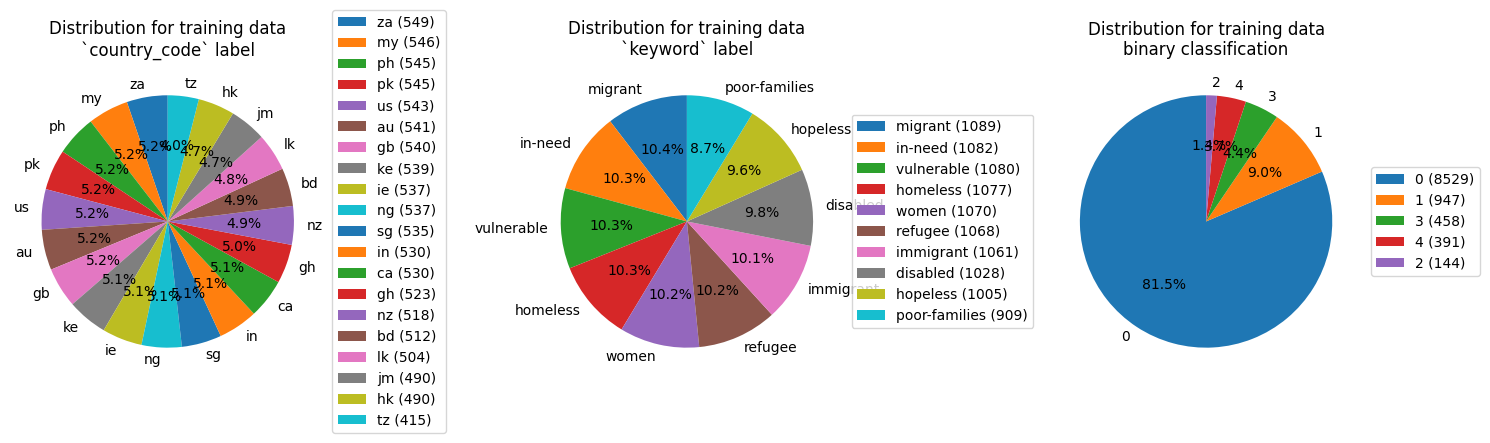
\includegraphics[trim=0cm 0cm 0cm 0cm, clip, width=\linewidth]{figures/test_distribution.png}
    \caption{Pie charts of different label distributions in the supplied dev-set}
    \label{fig:dev-set-distribution}
\end{figure*}

\begin{figure}[H]
    \centering
    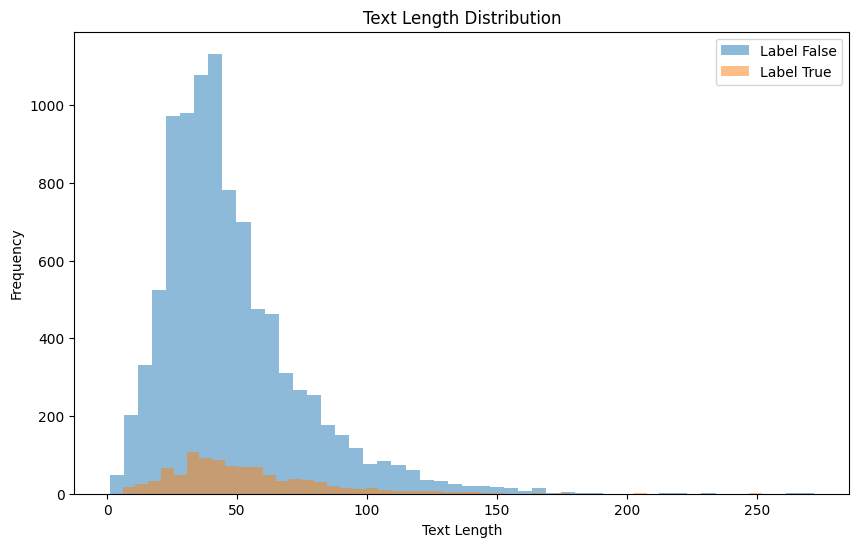
\includegraphics[trim=0cm 0cm 0cm .8cm, clip, width=\linewidth]{figures/text-input-length-by-binary-patronizing.png}
    \caption{Histogram of word count by PCL (true) and non PCL (false)\footnotemark}
    \label{fig:word-count}
\end{figure}

\footnotetext{Without loss of generality, text with more than 250 words have been clipped}

Furthermore, the distribution of word counts between the two (See Figure~\ref{fig:word-count}) offers no obvious underlying pattern between the two classes. This is because natural language is about how words are said, instead of the quantity. 

\subsection{Subjective Difficulty}

Indeed, \citet{perez-almendros-etal-2020-dont} mention the subjective nature of the task as it is very subjective. The word `lovely' appears uniquely in PCL text examples. This word isn't negative, but in the context of the sentence (par\_id: 2404) ``We think it's lovely that so many have come forward to help out a family clearly in need!'' the sentence has been labeled as blatantly PCL with a score of 3. In-fact, tweaking the sentence from ``a family clearly in need'' to ``families in need'' removes entitlement and converts it to compassion.

\subsection{Artifacts}\label{sect:artifacts}

The flexible environment of news articles allows for authors to post resources and further reading, like in the case of par\_id: 2838: \emph{``Read more about the site's history here: [LINK]''}. Therefore, with a primitive language processing model, we cannot determine the degree of PCL from a link. Some links and references are also clipped in the source with token ``TOOLONG'' which also aught to be pre-processed to avoid confusion from the model. Additionally, writers are free to reference other users (par\_id: 5598 ``@toekunbore [...]''), the handle of which would likely be ignored by language models.

Lastly, adding to the complexity of processing language, we must also filter and process out-of-vocabulary words. This may appear in the form of a typo like in par\_id: 8221 \emph{``Do they think it is "" \textbf{jsutice} "" \textbf{ti} imprison [...]''}, hyperboles like par\_id: 5333 \emph{``But \textbf{nooooo} [...]''}, or slang like in par\_id: 1674 \emph{``Kyle really your a pig, \textbf{lol} [...]''}.

% \textbf{10 marks}: Further model improvements (beyond using a bigger transformer model), for example pre-processing, data sampling, data augmentation, ensembling, etc. Two main improvements, with a third less explored improvement is sufficient. For example: try several different data sampling approaches, try several data augmentation strategies by perturbing observations in different ways, and then see if incorporating one of the categorical columns improves performance.

% \begin{itemize}
%     \item try and balance out the classes by applying synonyms to low frequency labels
%     \item data-sampling, research: is it common to feed in an equal proportion of each class in batches during training?
%     \item using country code also
% \end{itemize}

\section{Minority Upsampling}

The data is very imbalanced; Section~\ref{sect:feature-distribution} discusses the sparsity of positive PCL examples in the training data. Therefore, it is possible that the model may experience great performance in the majority negative class, and fail to learn details about the minority positive class (\citet{alberto-imbalanced-datasets}).

We can synthetically produce more data points for the minority positive class by changing the content of the sample without changing the sentiment of the text. 

\subsection{Failed Considerations}

All data augementations are equal, but some are more equal than others; throughout development, considerations for data augmentations were made, but not all were implemented.

\subsubsection{Stop Word Removal}

Stop words contain little value, so can useful to decrease the length of sentence. However, it may change the sentiment of a sentnece: ``I do not like you because I'm better than you'' changed into ``I like I'm better'', thus removing all PCL sentiment from the sentence, and rendering an innefective augmentation.

\subsubsection{Easy Data Augmentation}

\citet{wei-zou-2019-eda} propose a pipeline to tweak sentences by replacing, deleting, swapping and inserting words. The authors comment that by fine-tuning replacement parameters and the upsampling factor, it can ``can boost performance on text classification tasks''. However, we found that the model quickly overfit within one epoch.

\subsubsection{Rephrasing Models}

Further effots were dedicated to rephrasing the text with the help of a pre-trained GPT-2 model as suggested by \citet{Dai2023AugGPTLC}. However, significant inconsistencies were discovered depending on the sentence length, so ultimately this effort was abandoned.

\subsection{Successful Considerations}

\subsubsection{Translation}

This upsampling technique is inspired by \citet{nlp-imbalanced-data} who suggests trainslating the text into a non-english language and then back into English. The hope is that translating back introduces new wording and structure without augmenting the sentiment of the sentence. We take this a step further by introducing a parameter to control the depth of translation.

\subsubsection{Swapping Sentences}

Within the same paragraph, we can swap the ordering of sentences. This augmentation was less researched by helped upsample the minority class.

\section{Data Augmentation}

\subsection{Tokenization}

By tokenizing the input, we can efficiently assign \texttt{[UNKNOWN]} tokens to out-of-vocabulary words. This is important for a pre-trained model which are trained on well-formed English text, and may not understand slang or typos.

\subsection{Masking inputs}

Further benefit of tokenization includes the choice of randomly masking a subset of words in the input. This allows models to capture rich contextual information and dependencies in language. This allows the model to generalize well to various text classification tasks, even when faced with different writing styles, vocabulary, and sentence structures.

\section{Modelling}\label{sect:model}


\emph{For the successful implementation of a classifier model (this could be a transformer or any other ML model of your choice. Do give justification for your choice.):}

\subsection{Model Choice}

\textbf{10 marks}: Successful implementation of a model (train and produce predictions which outperform the F1 score for the RoBERTa-base baseline provided). 7 marks for outperforming the baseline model on the official dev set (0.48) and 3 marks for outperforming the baseline model on the test set (0.49).

\subsection{Hyper-parameters}

\textbf{5 marks}: Choice of model hyper-parameters and description of your model setup. This should include choosing an appropriate learning rate and checking whether implementing a learning schedule improves performance. Also consider whether your model is cased or uncased. You should mention how many epochs you train the model for, whether you are using any early-stopping, and how you are using the training labels.

\section{Results}

\textbf{5 marks}: Description of the model results and your hyper-parameter tuning (some evidence of this is required in your report). Your results should show how the different strategies you have tried impacted the model performance. For any results presented in your paper, you should be clear if these are from your own internal dev set or the official dev set.

\subsection{Comparison}

\textbf{10 marks}: Compare your model performance to two simple baselines (e.g. a BoW model). Share some of the features that one of your baseline models used, and highlight an example misclassified with a suggestion of why the baseline may have made the misclassification.

\section{Analysis}

\emph{Analysis questions to be answered (these questions can be answered without training any additional models): Your report should state the analysis questions so that this can be read as a self-contained report, rather than referring to ‘analysis question 1’ etc.}

\begin{enumerate}
    \item \textbf{5 marks}: To what extent is the model better at predicting examples with a higher level of patronising content? Justify your answer.
    \item \textbf{5 marks}: How does the length of the input sequence impact the model performance? If there is any difference, speculate why.
    \item \textbf{5 marks}: To what extent does model performance depend on the data categories? E.g. Observations for homeless vs poor-families, etc.
\end{enumerate}

\section{Conclusion}

\textbf{5 marks}: Conclusion, with a summary of your results, and your key
findings from the analysis questions. You should suggest at least one further
experiment as a next step.

\clearpage

\appendix

\bibliography{references}
\bibliographystyle{acl_natbib}

\end{document}
